\chapter{Background and State of the Art}
\label{ch:Background and State of the Art}

\section{Anomalies Detection Techniques}
According to \cite{article:15_survey_ad}, the task of outliers detection, which is a main objective task of this work, has been an object of interest and studies of research community originating from 19\up{th} Century. Nowadays a huge variety of different techniques for solving the task of detecting outliers and abnormalities in video traffic data are presented, and these approaches can be classified in various ways.

For example, data mining techniques in general and anomaly detection techniques as well as clustering approaches, which are one of the ways to solve the task of outliers identification, particularly can be classified as supervised, semi-supervised and unsupervised on the grounds of the manner of labeling the input data] \cite{article:15_survey_ad}:
\begin{enumerate}
	\item \textit{Supervised}. Input data used for training contains labels for both normal and anomalous instances. As a result the algorithm can build models for both normal and abnormal classes;
	\item \textit{Semi-Supervised \cite{article:15_survey_ad}} or \textit{Weakly-Supervised \cite{article:5_survey_tbsa}}. Input training data set contains class labels only for normal data instances. Such techniques are more widely used than supervised approaches, since anomalous data instances are usually not predictable and random and it is difficult to provide examples to cover all possible anomalous events;
	\item \textit{Unsupervised}. Does not require input data to be labeled neither for normal nor anomalous data. Such algorithms are based on the expectation that normal data instances are significantly more frequent than anomalous ones in the test data set and therefore are not applicable when this assumption is disrupted.
\end{enumerate}

Alternatively, according to surveys done by Chandola in \cite{article:15_survey_ad} and Kumaran in \cite{article:6_survey_anom_det_rtuvs}, anomaly detection techniques can be classification based, nearest-neighbor based, clustering based, statistical and etc. The following offers the short overview of mentioned groups.

\subsubsection{Classification based}
The main concept of these methods lies in using a classifier which firstly learns to distinguish inliers and outliers and then classifies each input instance \cite{inproceedings:18_ardod_lstd}. Such techniques consist of training and testing phases. Training, or learning, phase supposes learning a classifier model from a training data set, containing labeled data instances. The learned classifier is then used to classify an input trajectory as normal or anomalous by assigning a class label in a testing phase.

Depending on how testing data instances are labeled, all classification based anomaly detection techniques can be one-class or multi-class. The first type assumes that all training data instances are normal and are labeled as one class. During training phase model learns a discriminative boundary around normal instances, and a trajectory, which is not aligned with the learned normal class description, is considered as an anomalous. Single-class Support Vector Machines (SVMs) is the most commonly used classification based approach, which is applicable to the task of anomalous trajectory detection, as it was proposed by Piciarelli \textit{et al.} \cite{inproceedings:16_va_tad_svm}\cite{article:17_tbaed}. However, this approach requires trajectory vectors to be the same length. Since raw trajectory data is usually contains different amount of trajectory points due to different speed of moving objects, it is necessary to preprocess raw trajectories to normalize them to vectors of the same length \cite{article:17_tbaed}. Moreover, SVMs become highly time and memory consuming while working with huge amounts of multi-dimensional data \cite{article:22_survey_dscc}.

The latter category supposes learning multiple classes during training step and then using a classifier to review the input trajectory for compliance with each learned class. In literature different descriptions of training phase and training data labels are given. According to \cite{article:15_survey_ad}, training data contains only normal data instances with corresponding normal class labels, and during training phase model learns multiple discriminative boundaries around each class of normal instances. A trajectory, which is aligned with none of the learned normal class descriptions, is considered as an anomalous. In other words, an anomalous trajectory will not be accepted by neither of the classifiers. In \cite{article:6_survey_anom_det_rtuvs} it is assumed that model is learned using training data containing labels for normal and anomalous classes. Therefore, a classifier can classify an input trajectory as belonging to a normal or anomalous class.

The advantage of two-phased classification based algorithms is a fast testing phase due to precomputed classifier model used to classify each input instance. Also such algorithms can perform well in cases when anomalous data instances form a class or cluster \cite{inproceedings:18_ardod_lstd}. However, the training step requires accurately labeled training data, which is often not available. 

\subsubsection{Nearest-neighbor based \cite{article:15_survey_ad} or Proximity / Distance based \cite{article:6_survey_anom_det_rtuvs}\cite{inproceedings:18_ardod_lstd}}
Proximity based approaches decide whether a data instance is normal or anomalous based on how close or far is it located with respect to neighbors \cite{article:6_survey_anom_det_rtuvs}. Nearest-neighbor and density based approaches are based on the assumption, that «normal data instances have dense neighborhood, while anomalous data instances occur far from their closest neighbors» \cite{article:15_survey_ad}.

In order to be able to compare the surrounding density for an instance under consideration with the density around its local neighbors, a distance (dissimilarity) or similarity measure between two data instances needs to be specified \cite{inproceedings:18_ardod_lstd}. By virtue of an anomaly score calculation method, techniques can be grouped into two categories: 1) the anomaly score is calculated as a distance of a data instance to its $k^th$ nearest neighbor and 2) to compute the anomaly score the relative density of each data instance is being computed \cite{article:15_survey_ad}.

These approaches has several disadvantages. First of all, in comparison with classification based anomalies detection techniques, the computational complexity of the testing phase is considerably higher, since nearest neighbors are computed by computing the distance for each test data instance with all instances from either testing and training data. In case of multi-dimensional trajectory data, the task of distance computation becomes even more complicated. Moreover, the accuracy of labeling decreases when the main assumption is violated: when normal instances have sparse neighborhood or anomalous instances have dense \cite{article:15_survey_ad}.

\subsubsection{Clustering based}
Clustering is an efficient approach aimed to group data instances into different classes, called clusters, based on their similarity in such a way, that objects in one cluster are similar to each other and dissimilar to objects in other clusters \cite{article:8_review_mot_cl_alg}\cite{article:22_survey_dscc}. ST clustering supposes grouping objects on the ground of their spatial and temporal similarity. To compare data instances before grouping them into clusters, similarity or distance between them needs to be measured.

There are three types of clustering based anomalies detection techniques with following assumptions: 1) normal data instances are associated with a cluster, while anomalous data instances are not associated with any cluster, 2) normal data instances are close to the cluster center, while abnormal instances lie far away from the closest cluster center and 3) normal data instances lie in large and dense clusters, while anomalies are associated with sparse clusters or clusters with a small cardinality \cite{article:15_survey_ad}\cite{article:6_survey_anom_det_rtuvs}. Techniques of first type can be implemented using one of the clustering methods which do not require every data instance to belong to some cluster, for example DBSCAN \cite{inproceedings:20_dbscan}. Algorithms from second group consist of two phases: 1) data clustering and 2) calculating an anomaly score for each data instance. Techniques of the latter type require a threshold for cardinality size and/or density of a cluster to be defined to decide whether a cluster refers to normal or anomalous data.

The necessity to compute distance between trajectories in some of the clustering based approaches makes them similar to neighbor based approaches. As it is stated in \cite{article:15_survey_ad}, techniques are different in the way they process instances: in clustering based techniques each instance is evaluated with respect to the corresponding cluster, while in neighbor based techniques each instance is being inspected with respect to its proximate neighborhood. Consequently, the selection of distance computation method plays an important role and affects results and performance significantly.

On the other side, dividing all training data into groups makes clustering based algorithms similar to classification based algorithms. Though in classification based approaches class is assigned based on given labels, while in clustering based approaches classification is not given in advance \cite{inproceedings:18_ardod_lstd}.

One of the main advantages of clustering based techniques is the ability of majority of them to run in an unsupervised manner. For the case of TVS-based trajectory data acquisition the unsupervised learning methods are the most appropriate, because labeling hours of video data is a highly time-consuming task. Also, manual labeling of input data can lead to errors due to human operator intervention.

Moreover, clustering based techniques are adjustable to work with complex data types because of adaptability of clustering algorithms. However, at the same time they are computationally expensive, highly dependent on the used clustering algorithm and can not effectively deal with situations when anomalies form significant separate cluster groups \cite{article:15_survey_ad}.

\subsubsection{Model based \cite{article:6_survey_anom_det_rtuvs}\cite{inproceedings:18_ardod_lstd} or statistical \cite{article:15_survey_ad}}
The main concept of model based algorithms is that they represent the data as a set of parameters to create the model of a normal behavior. Statistics based approaches can be considered as a subcategory of model based approaches. As it is stated in \cite{article:15_survey_ad}, the main idea of statistical approaches is that data instances occurring in high probability regions of a stochastic model assumed to be normal, while data instances from the low probability regions refer to anomalies. So, statistical approaches are based on using statistical stochastic model to fit to the given data and then applying a statistical inference test, also called discordance test, to decide if a data instance is normal or anomalous. It comes from the main concept that «based on results of applied statistical test, anomalies have low probability to be generated from the learned stochastic model» \cite{article:15_survey_ad}.

Statistical techniques in turn can be parametric or non-parametric. In parametric approaches the normal data is supposed to fit the parametric distribution and probability density function with estimated from the given data parameters \cite{article:6_survey_anom_det_rtuvs}. However, it is difficult to fit the data to one distribution. In this case it is possible to use a multiple-distribution model to match some clusters of the data with particular distributions \cite{inproceedings:18_ardod_lstd}. By contrast to this, non-parametric approaches are based on using non-parametric statistical models with structures, which are not defined in advance: the given data is used to determine the structure dynamically.

Since statistical approaches are based on fitting a statistical model, the choice of it significantly affects results, computational complexity and performance. Nevertheless, the main assumption of statistical approaches that the data comes from a particular distribution can not be always satisfied, specifically for the case of a multi-dimensional data \cite{article:15_survey_ad}.

\subsubsection{Summary}
Based on the given description of different approaches and their advantages and disadvantages, it was decided to focus on clustering based anomalies detection approaches for several reasons: 
\begin{enumerate}[label=\arabic*)]
	\item they can work in an unsupervised mode without a human intervention and do not require the input data to contain labels,
	\item input data is allowed to contain anomalous trajectories,
	\item clustering method can be easily applied to such a multi-dimensional data as trajectories by defining a suitable similarity measure.
\end{enumerate}

That means that a clustering method and a similarity measure need to be specified.

\section{Clustering Approaches}
Clustering is a highly researched form of data mining, and huge variety of clustering methods has already been proposed in literature \cite{article:8_review_mot_cl_alg}. State-of-the-art analysis of related research papers revealed that all traditional clustering approaches are usually categorized into five types: partitioning, hierarchical, density-based, model-based and grid-based methods \cite{article:5_survey_tbsa}\cite{article:8_review_mot_cl_alg}. Next paragraphs will briefly discuss each of the categories with highlighting main assumptions and concepts.

\subsubsection{Partitioning, or Partition-based, methods}
Such methods are based on partitioning the trajectories data set randomly and then regrouping clusters by reassigning objects from one partition to another to minimize the objective function. They require the predefined parameter, usually denoted as $k$, which determines the amount of final clusters, or partitions, to be created. The main requirement is that number of partitions must be smaller than number of initial data points, since each partition forms a cluster, that means that it must be non-empty and contain at least one data instance, and each data instance must be included into exactly one cluster.

One of the most well-known examples of partitioning clustering algorithms is a $K$-Means algorithm, where firstly $k$ cluster centers are initialized randomly and then data points are iteratively reassigned to the closest clustering center based on the discrepancy to minimize the clustering error \cite{article:23_survey_ca}. The clustering error is defined as the sum of the squared Euclidean distances between each data set point and the corresponding cluster center \cite{article:24_glkkm_cl_fs}. The process is stopped when there are no more changes in clustering centers.

The disadvantages of the traditional K-Means clustering method are inability to form clusters of arbitrary form, dependence on initial random cluster centers initialization and high memory consumption \cite{article:8_review_mot_cl_alg}. Also finding an appropriate partitioning technique is a challenging task.

\subsubsection{Hierarchical methods}
In hierarchical based methods the given data set is decomposed into multiple levels to organize a hierarchical tree of clusters. The resulting hierarchical structure can be depicted as a tree \cite{article:23_survey_ca}.

There are two different ways of hierarchical decomposition: 1) the bottom-up (combining) and 2) the top-down (split, divisive) decomposition. They refer to agglomerative and divisive (split) clustering approaches respectively. Agglomerative hierarchical clustering algorithms start by assigning each data instance to a distinct singleton-cluster, so the number of initial clusters is equal to the exact amount of data instances in input data, and then continue uniting clusters based on theirs similarity. Proximity matrix is used to store similarity measurements between clusters and is being updated on each step by computing distances between the new cluster and the other clusters. The divisive hierarchical clustering algorithms work in a reverse manner: initially all data instances belong to one cluster and then step by step clusters split into smaller clusters until all of them become singleton clusters or until satisfying some predefined end condition.

Hierarchical clustering is supposed to be simple, but it is necessary to choose between agglomerative and split methods. Divisive clustering is more expensive in computation, therefore, it is less common than agglomerative approaches. Irreversibility of both splitting or uniting processes in traditional hierarchical clustering algorithms is also a particularity of such algorithms \cite{article:8_review_mot_cl_alg}.

Since approach includes clusters joining, a significant task of agglomerative clustering algorithms is defining and computing the similarity or distance between clusters. This similarity can also be referred to as an inter-cluster or between-cluster distance. For the case of single-trajectory clusters the similarity between them is simplified and is equal to the similarity between respective trajectories. For multiple-trajectory clusters the similarity is computed according to a chosen linkage method. In literature following linkage methods are given as mostly common: single link, complete link, average link \cite{article:23_survey_ca}\cite{inproceedings:7_related_work}. In the case of the single link distance between two clusters is defined as the minimum distance between two trajectories in these clusters, that means that the similarity between of two clusters is determined by two closest trajectories. The complete link linkage method implies taking the maximum distance between two trajectories in two clusters as an inter-cluster distance, so it is defined using the farthest distance of trajectory pairs. The average link supposes calculating averaged paired distance between all trajectory pairs in these two clusters.

A convenience of agglomerative hierarchical clustering approaches is that they do not require the number of resulting clusters to be predefined, so they are appropriate for clustering vehicle trajectories, because number of clusters of normal or anomalous trajectories is not known in advance. However, the most well-known disadvantage of hierarchical clustering algorithms is that they are not robust and can suffer from noise and anomalies. 

\subsubsection{Density-based methods}
In comparison with the partitioning and hierarchical clustering approaches, density-based methods objects inspect similarity based on the density of the data \cite{article:22_survey_dscc}. The area is being added to the nearest cluster, while density of the points in the area remains greater than the predefined threshold \cite{article:8_review_mot_cl_alg}. Clusters form dense regions of objects and they are separated by sparse regions with low density.

The main advantage of density-based clustering approaches is that they are able to form clusters of arbitrary forms, extend beyond spherical \cite{article:8_review_mot_cl_alg}. Also they are appropriate for clustering huge data sets of trajectories in an unsupervised manner and do not require the amount of clusters to be known in advance \cite{article:5_survey_tbsa}\cite{article:22_survey_dscc}. However, the results quality highly dependent on the amount of trajectories in training data set, available for analysis.

The most well-known and commonly used density-based algorithm is a DBSCAN, proposed by M. Ester \textit{et al.} in \cite{inproceedings:20_dbscan}. According to it, input data points are categorized as follows: core data, density-reachable data and outliers based on parameters $\varepsilon$, \textit{minPts} and the density threshold. Neighbor parameter $\varepsilon$ and \textit{minPts} specify the maximum remoteness and minimum amount of satisfying points while choosing the core points: at least \textit{minPts} points must be present within distance $\varepsilon$ from the core point, these points are marked as directly reachable from the chosen core point. Aforementioned parameters need to be predefined by the user, but it is difficult to determine them correctly. Each cluster must contain at least one core point. Points are denoted as anomalous if they are not reachable from any of the other points.

\subsubsection{Shrinkage-based or Grid-based methods}
The main idea of grid-based algorithms lies in applying a multi-resolution grid data structure: the data space is quantized into a finite number of cells (units) that form a multi-resolutional grid structure. Each cell stores summary information about data objects within its subspace \cite{article:22_survey_dscc}. Since clustering operations are performed on the created grid, and also important trajectories characteristics can be computed in each of the spatial grid cells, the quality of data compression influences the quality of results significantly \cite{article:1_survey_stdm}. Density of closely located dense cells can help to determine clusters. A trajectory can be considered as an anomalous if it differs from the expected trajectory in a number of covered grid cells \cite{article:22_survey_dscc}.

The main advantage of grid-based clustering algorithms is an improved performance: increased processing speed and processing time becomes independent on the size of the data set, only the number of cells in each dimension in the quantized space affects the processing time \cite{article:8_review_mot_cl_alg}.

\subsubsection{Model-based methods}
In comparison with the above methods, which analyze distance among data objects, in model-based approaches data is supposed to be generated by a mixture of probability distributions, where each component of mixture represents a cluster. So a mathematical model is assigned to each cluster, and then method attempts to find the best fitting data for the chosen model. In this way such methods seek to increase the adaptability between given data and some statistical models \cite{article:8_review_mot_cl_alg}\cite{article:22_survey_dscc}. The idea of model-based algorithms is that in order to locate clusters they describe the spatial distribution of the input data points by building density functions. The model-based approaches are typically used in feature-specific clustering and depend on the selected features and model \cite{article:5_survey_tbsa}.

It is emphasized, that model-based approaches show good performance while working with complex data types. This category usually includes statistical and neural network methods \cite{article:8_review_mot_cl_alg}.

\subsubsection{Graph-based methods \cite{article:1_survey_stdm}}
Another category of clustering methods in application to vehicle trajectories data. Liu \textit{et al.} in \cite{inproceedings:26_dstci_tds} presented a graph-based approach to solve the problem of detection of outliers in traffic data streams. A graph structure was used to store the traffic: nodes represent regions while edge weights depict the traffic flow. Edge anomalies in the graph denote the traffic abnormalities, and causal outlier tree can then be used to further analyze these outliers to find causal interactions.

\bigbreak
Another higher-level classification of clustering methods can consist of only two sub-classes on the ground of properties of generated clusters: hierarchical and partitioning approaches \cite{article:23_survey_ca}. Hierarchical algorithms group objects into clusters from singleton cluster to cluster containing all data instances or in a reverse direction. While partitioning clustering algorithms divide given data set into a predefined number of clusters in a single-layer structure.

In order to perform clustering, the similarity between two trajectories needs to be defined. Different existing distance measures will be reviewed in following paragraphs.

\section{Distance and Similarity Measures}
As it was mentioned before, clustering based approaches require a similarity measure to be defined between two trajectories. Apart from that, distance and similarity measures are also used to compare a trajectory with a cluster or a pair of clusters between each other. A similarity measure highly dependent on the format of a trajectory. A trajectory data, represented as a multidimensional data, can contain quantitative or qualitative features, continuous or binary. In such a classification, distance measure functions are more appropriate to work with continuous features, while similarity measures – with qualitative features \cite{article:23_survey_ca}. Input trajectory-vectors in this work contain spatial information along with temporal, which can be termed as qualitative continuous data. That means that distance measure functions are more appropriate in this case. Moreover, distance and similarity functions can be classified as 1) working with raw representations of trajectories without any preprocessing steps and 2) working with preprocessed trajectories representations. Preprocessing can include unifying the length of trajectories or reducing the dimensionality of trajectory-vectors \cite{inproceedings:7_related_work}. 

Some of the most known, widely used traditional similarity measures are following: Euclidean distance, Fréchet Distance, DTW, LCSS.

\subsubsection{Euclidean distance}
Euclidean distance between two trajectory vectors is calculated as a sum of squared differences of corresponding spatial coordinates \cite{article:27_vna_cad_td}:
\begin{equation}
	 d_{ij} = ||T_i - T_j||_E = \sqrt{\sum_{k=1}^{m}((t_{i_x}^k - t_{i_x}^k)^2 + (t_{i_y}^k - t_{j_y}^k)^2)},
\end{equation}
where both trajectories consist of \textit{m} tracking points and are represented by two-dimensional vectors $T_i = \{t_i^1, t_i^2, \ldots, t_i^m\}$ and $T_j = \{t_j^1, t_j^2, \ldots, t_j^m\}$. Tuples $(t_{i_x}^k, t_{i_y}^k)$ represent spatial coordinates for a \textit{k}-th tracking point of \textit{i}-th trajectory from a data set.

However, Euclidean distance works only with trajectories with equal number of tracking points. Since usually vehicles move with different speed and behavior, trajectory length is always different and that means that raw trajectories need to be preprocessed and reduced to the same size \cite{inproceedings:7_related_work}. Also, traditional Euclidean distance requires two-dimensional data, meaning that it is not able to process temporal information, and is dependent on the trajectory direction: the reversed direction can cause incorrect distance measurement, that in its turn leads to errors in clustering. Also, it fails while working with trajectories moving in a similar way but with different speeds and in the case of different sampling rates \cite{inproceedings:28_lcss_dsmt}.

\subsubsection{Fréchet Distance}
Fréchet Distance is based on Euclidean distance. It considers the positional and sequential relationship of trajectory points while calculating the similarity. The main idea of this approach is computing Euclidean distance for each pair of points from two trajectories and then designating the maximum Euclidean distance as a Fréchet Distance between them \cite{article:8_review_mot_cl_alg}\cite{inproceedings:29_fr_dist}. However, since only the maximum among distance is considered, the approach is sensitive to the presence of outliers.

\subsubsection{DTW}
Dynamic Time Warping (DTW) is one of the algorithms for measuring the similarity between two temporal time series sequences, which may vary in speed. The objective of time series comparison methods is to produce a distance metric between them two. DTW method aims to find an alignment between time-dependent sequences, such as trajectories, and is able to process trajectories of different lengths \cite{article:8_review_mot_cl_alg}. 

According to \cite{article:8_review_mot_cl_alg}, DTW distance is calculated as follows (Formula \ref{eq:dtw}):

\begin{equation} \label{eq:dtw}
	D_D(T_i, T_j) = 
		\begin{cases}
			0 				&\text{m = n = 0}\\
			\infty 			&\text{m = 0 || n = 0}\\
			dist(a_i^k, b_j^k) + min 
				\begin{cases}
					D_D(Rest(T_i), Rest(T_j))\\
					D_D(Rest(T_i), T_j)\\
					D_D(T_i, Rest(T_j))
				\end{cases} &\text{others}
		\end{cases}
\end{equation}

where $D_D(T_i, T_j)$ refers to DTW distance between two trajectory segments with lengths $m$ and $n$, $dist(a_i, b_j)$ means the Euclidean Distance between two trajectory points. Function $Rest(T_i)$ takes the remaining part of a trajectory after excluding the point $a_i$. It can be seen, that in case of zero-length trajectories the DTW distance is equal to 0, for the case then only one of two trajectories is non-empty, the distance between them is considered to be infinite. For two non-empty trajectories, the minimum distance between them is calculated in a recursive way.

Though the important advantage of the DTW method is its ability to process trajectory vectors of distinct lengths, DTW distance is not robust to noise and requires trajectory points to be continuous. Also DTW distance computation is highly time consuming and complex due to necessity to compare distances between each pair of trajectories.

\subsubsection{LCSS}
Longest Common SubSequence (LCSS) distance tries to match two trajectory sequences based on the longest common sub-sequence between them. The task of finding the longest common sub-sequence is usually solved recursively \cite{article:8_review_mot_cl_alg}. The basic idea of an LCSS distance is that it allows two trajectories to stretch. In comparison with DTW and Euclidean distances, LCSS enables some elements to remain unmatched.

The LCSS distance is calculated according to the Formula \ref{eq:dlcss} \cite{inproceedings:7_related_work}:

\begin{equation} \label{eq:dlcss}
	D_{LCSS}(T_1, T_2) = 1 - LCSS_{\delta, \epsilon}(T_1, T_2) / min(m, n)
\end{equation}

where $m$ and $n$ are lengths of trajectories $T_1$ and $T_2$ respectively. The $LCSS_{\delta, \epsilon}(T_1, T_2)$, the longest common sub-sequence between trajectories, represents the number of matched trajectory points between trajectories $T_1$ and $T_2$ and is defined as follows (Formula \ref{eq:lcss}):

\begin{equation} \label{eq:lcss}
	LCSS_{\delta, \epsilon}(T_1, T_2) = 
		\begin{cases}
			0 			&\text{if m = 0 or n = 0}\\
						&\text{(if $|t_{1_{x,m}} - t_{2_{x,n}}| \textless \epsilon$}\\
			1 + LCSS_{\delta, \epsilon}(Rest(T_1), Rest(T_2)) 
						&\text{and $|t_{1_{y,m}} - t_{2_{y,n}}| \textless \epsilon$ }\\
						&\text{and $|m - n| \le \delta$)}\\
			max
			\begin{cases}
				LCSS_{\delta, \epsilon}(Rest(T_1), T_2)\\
				LCSS_{\delta, \epsilon}(T_1, Rest(T_2))
			\end{cases} &\text{otherwise}
		\end{cases}
\end{equation}

As it can be seen, LCSS calculation depends on two constant parameters: $\delta$ and $\epsilon$. Parameter $\delta$ defines \textit{the maximum remoteness in terms of time between two trajectory points in which we can look to match a given point from one trajectory with another}. Constant $\epsilon$ can take value between 0 and 1 and defines the size of proximity to look for matches in terms of spatial information. Difference between $X-$ and $Y-$coordinates less than $\epsilon$ value means that points are relatively close to each other and can be considered as similar. LCSS distance is increased by 1 in this case. Parameters $\delta$ and $\epsilon$ affect results significantly, therefore, the task of choosing the optimal values for them is challenging and important \cite{inproceedings:7_related_work}\cite{inproceedings:28_lcss_dsmt}. The $Rest(T)$ function is defined to return the last $M - 1$ points from the trajectory $T$.

The LCSS distance is the most appropriate in this work, since it allows the trajectories to contain noise, have different length, objects speed and sampling rates (local time shifts in trajectories) \cite{inproceedings:7_related_work}. Moreover, among the aforementioned methods, the LCSS distance is the most robust approach against noises.


\section{Related Work}
The aforementioned objective has been investigated and solved in numerous works using different methods. Since in fact normal events are common and dominate the data, and abnormal events are rare and difficult to describe explicitly, many approaches are based on an unsupervised clustering of trajectories. For this thesis work the approach proposed by Ghrab, Fendri, Hammami in \cite{inproceedings:7_related_work} was chosen as a basis. It is focused on detection of abnormalities based on a trajectories clustering.

The proposed approach consists of two phases (\ref{fig:str}):
\begin{itemize}
	\item \textit{offline} to perform clustering and extract frequent trajectories, and
	\item \textit{online} to classify the new trajectory as a normal or abnormal one.
\end{itemize}
\begin{figure}[!htb]
	\centering{}
	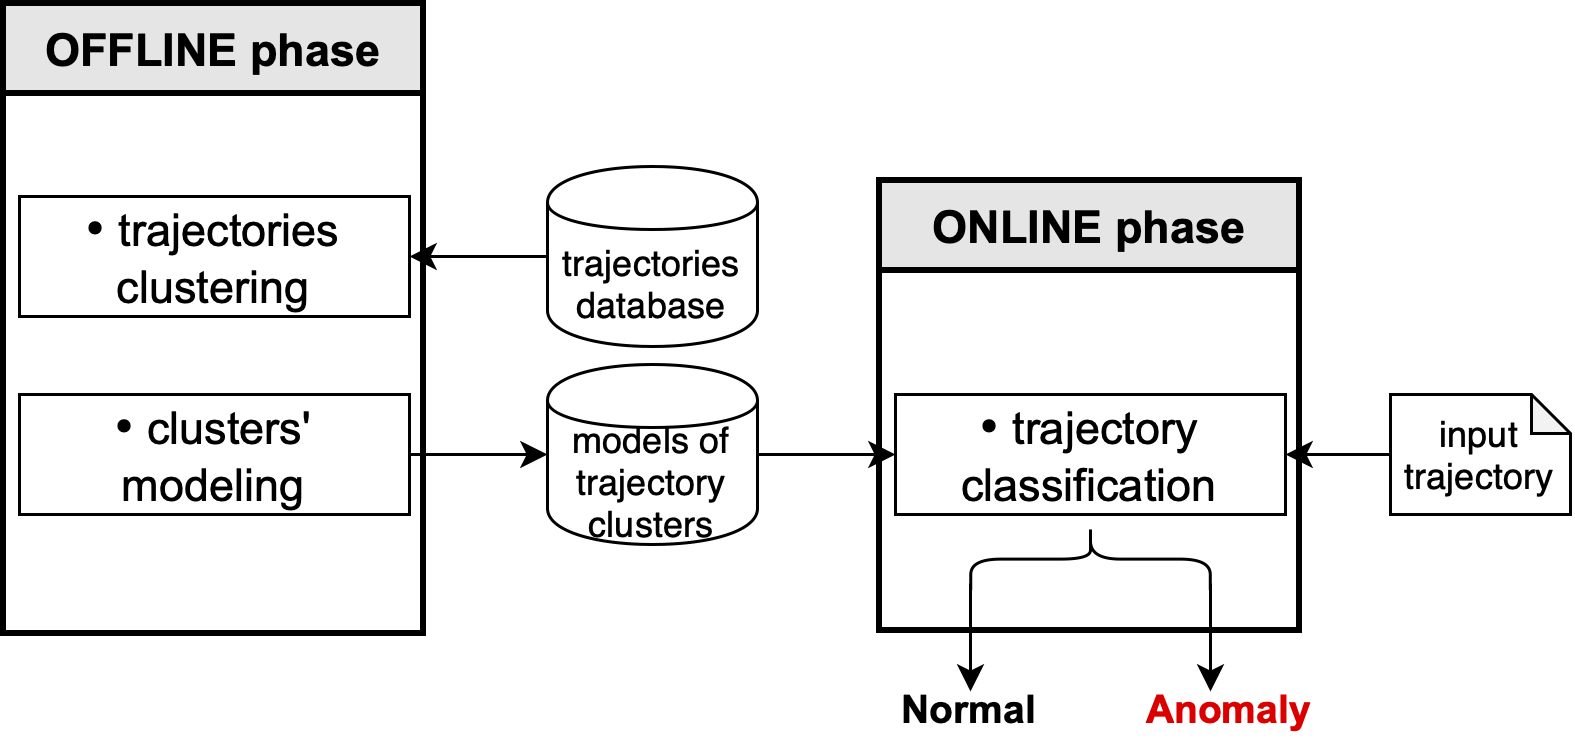
\includegraphics[width=0.8\textwidth]{images/str.png}
	\caption{Two-phased proposed approach}
	\label{fig:str}
\end{figure}

The clustering is done in an unsupervised manner using an agglomerative hierarchical clustering algorithm operating on a distance matrix between trajectories. To perform clustering, the LCSS distance is used as a similarity measure. The formulas and description of the LCSS distance are given in the previous section (Formulas \ref{eq:dlcss} -- \ref{eq:lcss}).

As it was already mentioned, hierarchical agglomerative clustering methods suppose clusters joining, which requires the inter-cluster distance measure to be defined. In \cite{inproceedings:7_related_work} authors have performed evaluation of different linkage methods, including single link, complete link and average link. According to the performed tests, the single link method showed the best results and, in view of this, will be used as a linkage method in the current work.

Single link linkage method considers a minimum distance between two trajectories as an inter-cluster distance and can be summed up as \cite{inproceedings:7_related_work}:

\begin{equation} \label{eq:single_link}
	D_{min}(C_i, C_j) = \min_{T_1 \in C_i, T_2 \in C_j} D_{LCSS}(T_1, T_2),
\end{equation} 

where ($C_i$, $C_j$) denote two clusters and ($T_1$, $T_2$) correspond to two trajectories from two clusters respectively.

\subsubsection{Advantages}
One of the advantages of the proposed method is that the chosen similarity measure does not require the trajectories to be of the same length, so that the preprocessing of the trajectories, which is a high complexity process, can be avoided. Moreover, the training data is allowed to contain normal trajectories as well as anomalous: algorithm will extract both normal and anomalous clusters. Dense clusters will represent normal trajectories classes, sparse clusters – anomalous trajectories classes.

\subsubsection{Disadvantages}
However, the disadvantage of the proposed method is that LCSS distance does not take into consideration such problems of video surveillance as a view perspective and a position of a moving object. 

\subsubsection{Summary}
This thesis work will be intended to investigate an opportunity of increasing the accuracy of results by making epsilon and sigma parameters, which are used to calculate the sigma, adaptable and dependent on the perspective and a distance from the camera. This includes:
\begin{itemize}
	\item exploring a functional dependency between epsilon and sigma parameters and a distance from the camera,
	\item evaluating algorithm with different values.
\end{itemize}